\documentclass[1p]{elsarticle_modified}
%\bibliographystyle{elsarticle-num}

%\usepackage[colorlinks]{hyperref}
%\usepackage{abbrmath_seonhwa} %\Abb, \Ascr, \Acal ,\Abf, \Afrak
\usepackage{amsfonts}
\usepackage{amssymb}
\usepackage{amsmath}
\usepackage{amsthm}
\usepackage{scalefnt}
\usepackage{amsbsy}
\usepackage{kotex}
\usepackage{caption}
\usepackage{subfig}
\usepackage{color}
\usepackage{graphicx}
\usepackage{xcolor} %% white, black, red, green, blue, cyan, magenta, yellow
\usepackage{float}
\usepackage{setspace}
\usepackage{hyperref}

\usepackage{tikz}
\usetikzlibrary{arrows}

\usepackage{multirow}
\usepackage{array} % fixed length table
\usepackage{hhline}

%%%%%%%%%%%%%%%%%%%%%
\makeatletter
\renewcommand*\env@matrix[1][\arraystretch]{%
	\edef\arraystretch{#1}%
	\hskip -\arraycolsep
	\let\@ifnextchar\new@ifnextchar
	\array{*\c@MaxMatrixCols c}}
\makeatother %https://tex.stackexchange.com/questions/14071/how-can-i-increase-the-line-spacing-in-a-matrix
%%%%%%%%%%%%%%%

\usepackage[normalem]{ulem}

\newcommand{\msout}[1]{\ifmmode\text{\sout{\ensuremath{#1}}}\else\sout{#1}\fi}
%SOURCE: \msout is \stkout macro in https://tex.stackexchange.com/questions/20609/strikeout-in-math-mode

\newcommand{\cancel}[1]{
	\ifmmode
	{\color{red}\msout{#1}}
	\else
	{\color{red}\sout{#1}}
	\fi
}

\newcommand{\add}[1]{
	{\color{blue}\uwave{#1}}
}

\newcommand{\replace}[2]{
	\ifmmode
	{\color{red}\msout{#1}}{\color{blue}\uwave{#2}}
	\else
	{\color{red}\sout{#1}}{\color{blue}\uwave{#2}}
	\fi
}

\newcommand{\Sol}{\mathcal{S}} %segment
\newcommand{\D}{D} %diagram
\newcommand{\A}{\mathcal{A}} %arc


%%%%%%%%%%%%%%%%%%%%%%%%%%%%%5 test

\def\sl{\operatorname{\textup{SL}}(2,\Cbb)}
\def\psl{\operatorname{\textup{PSL}}(2,\Cbb)}
\def\quan{\mkern 1mu \triangleright \mkern 1mu}

\theoremstyle{definition}
\newtheorem{thm}{Theorem}[section]
\newtheorem{prop}[thm]{Proposition}
\newtheorem{lem}[thm]{Lemma}
\newtheorem{ques}[thm]{Question}
\newtheorem{cor}[thm]{Corollary}
\newtheorem{defn}[thm]{Definition}
\newtheorem{exam}[thm]{Example}
\newtheorem{rmk}[thm]{Remark}
\newtheorem{alg}[thm]{Algorithm}

\newcommand{\I}{\sqrt{-1}}
\begin{document}

%\begin{frontmatter}
%
%\title{Boundary parabolic representations of knots up to 8 crossings}
%
%%% Group authors per affiliation:
%\author{Yunhi Cho} 
%\address{Department of Mathematics, University of Seoul, Seoul, Korea}
%\ead{yhcho@uos.ac.kr}
%
%
%\author{Seonhwa Kim} %\fnref{s_kim}}
%\address{Center for Geometry and Physics, Institute for Basic Science, Pohang, 37673, Korea}
%\ead{ryeona17@ibs.re.kr}
%
%\author{Hyuk Kim}
%\address{Department of Mathematical Sciences, Seoul National University, Seoul 08826, Korea}
%\ead{hyukkim@snu.ac.kr}
%
%\author{Seokbeom Yoon}
%\address{Department of Mathematical Sciences, Seoul National University, Seoul, 08826,  Korea}
%\ead{sbyoon15@snu.ac.kr}
%
%\begin{abstract}
%We find all boundary parabolic representation of knots up to 8 crossings.
%
%\end{abstract}
%\begin{keyword}
%    \MSC[2010] 57M25 
%\end{keyword}
%
%\end{frontmatter}

%\linenumbers
%\tableofcontents
%
\newcommand\colored[1]{\textcolor{white}{\rule[-0.35ex]{0.8em}{1.4ex}}\kern-0.8em\color{red} #1}%
%\newcommand\colored[1]{\textcolor{white}{ #1}\kern-2.17ex	\textcolor{white}{ #1}\kern-1.81ex	\textcolor{white}{ #1}\kern-2.15ex\color{red}#1	}

{\Large $\underline{12n_{0853}~(K12n_{0853})}$}

\setlength{\tabcolsep}{10pt}
\renewcommand{\arraystretch}{1.6}
\vspace{1cm}\begin{tabular}{m{100pt}>{\centering\arraybackslash}m{274pt}}
\multirow{5}{120pt}{
	\centering
	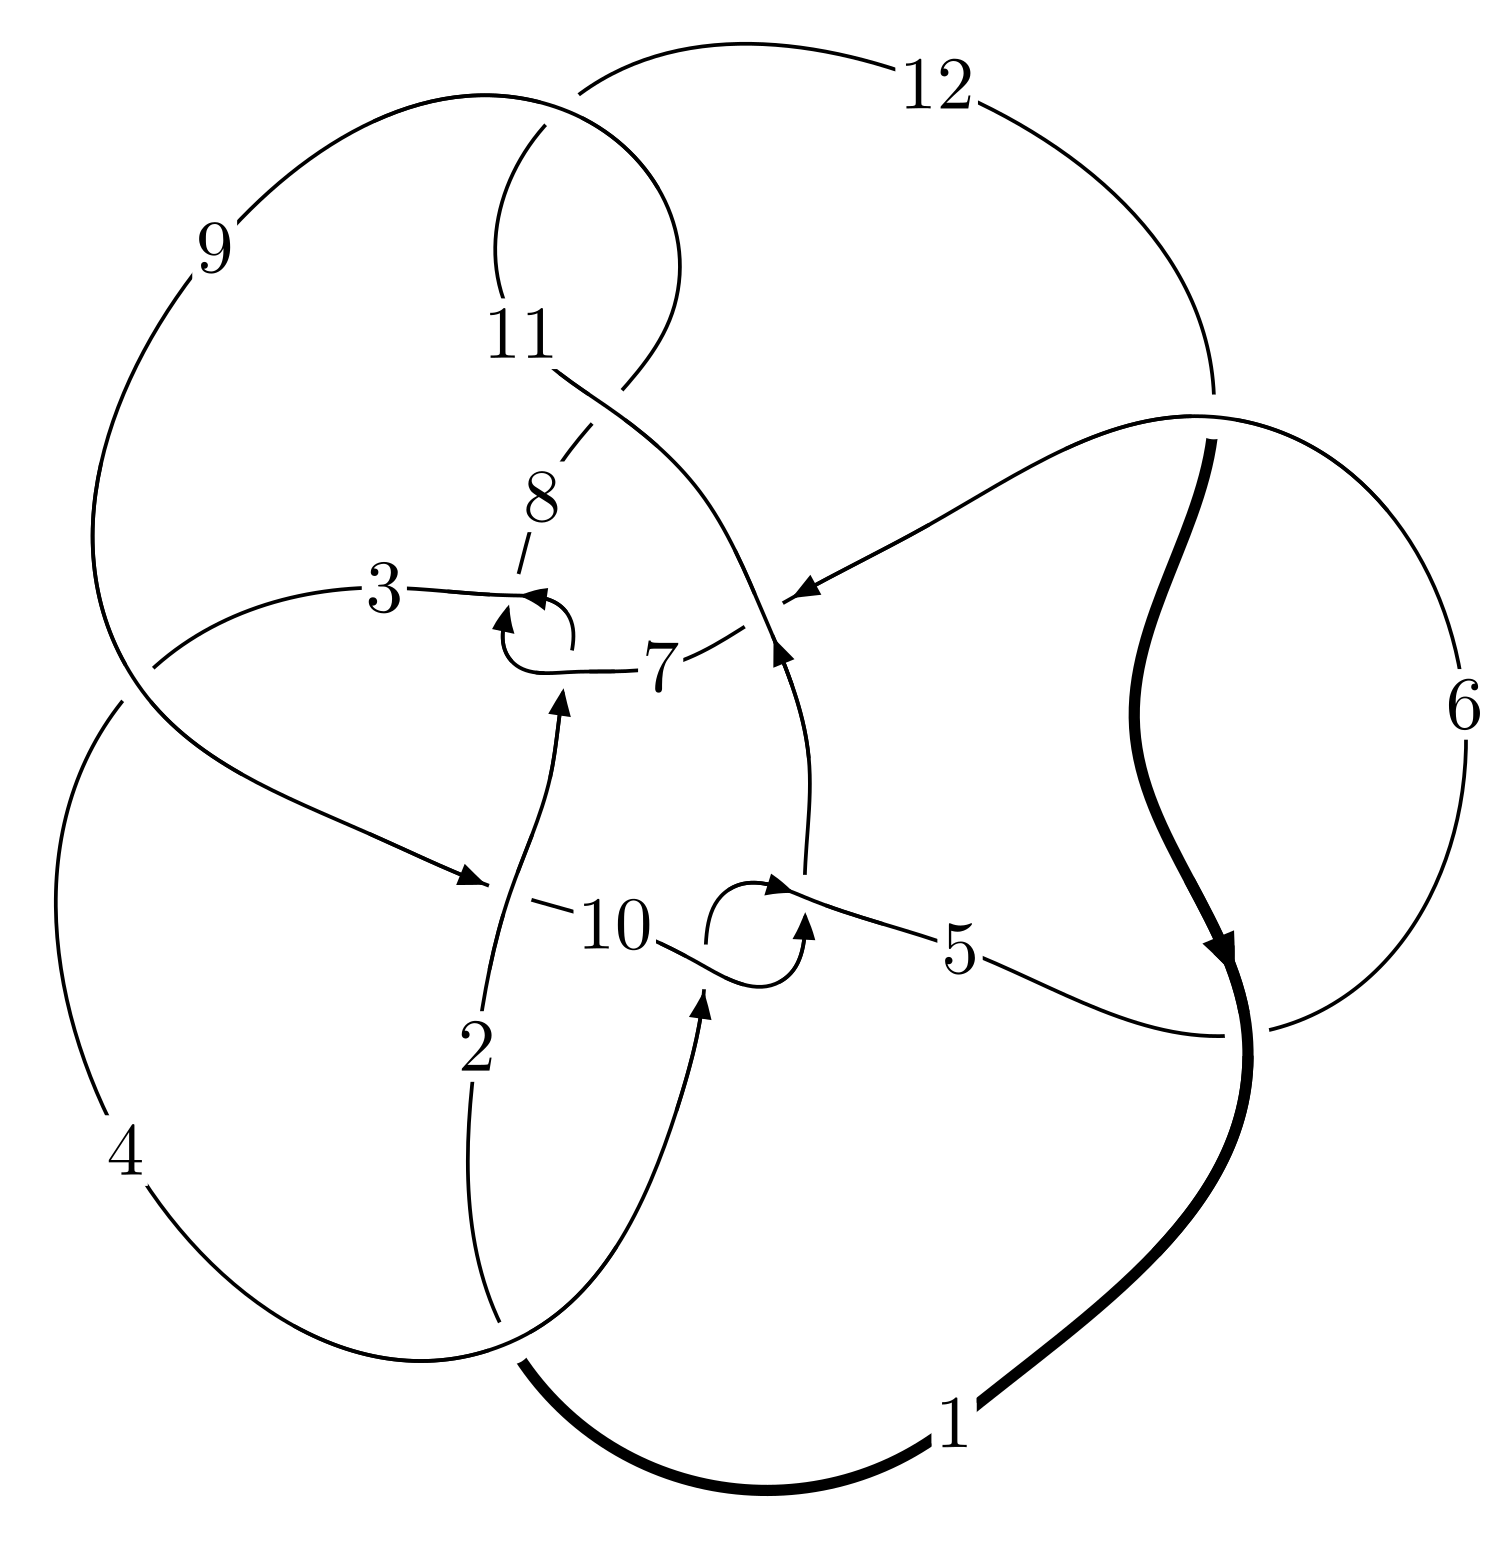
\includegraphics[width=112pt]{../../../GIT/diagram.site/Diagrams/png/2942_12n_0853.png}\\
\ \ \ A knot diagram\footnotemark}&
\allowdisplaybreaks
\textbf{Linearized knot diagam} \\
\cline{2-2}
 &
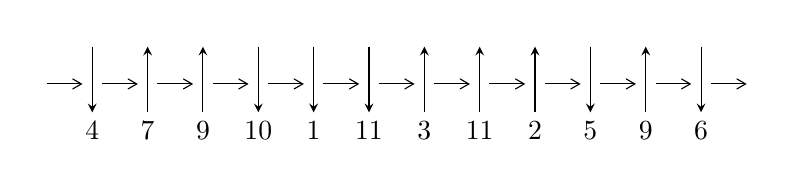
\begin{tikzpicture}[x=20pt, y=17pt]
	% nodes
	\node (C0) at (0, 0) {};
	\node (C1) at (1, 0) {};
	\node (C1U) at (1, +1) {};
	\node (C1D) at (1, -1) {4};

	\node (C2) at (2, 0) {};
	\node (C2U) at (2, +1) {};
	\node (C2D) at (2, -1) {7};

	\node (C3) at (3, 0) {};
	\node (C3U) at (3, +1) {};
	\node (C3D) at (3, -1) {9};

	\node (C4) at (4, 0) {};
	\node (C4U) at (4, +1) {};
	\node (C4D) at (4, -1) {10};

	\node (C5) at (5, 0) {};
	\node (C5U) at (5, +1) {};
	\node (C5D) at (5, -1) {1};

	\node (C6) at (6, 0) {};
	\node (C6U) at (6, +1) {};
	\node (C6D) at (6, -1) {11};

	\node (C7) at (7, 0) {};
	\node (C7U) at (7, +1) {};
	\node (C7D) at (7, -1) {3};

	\node (C8) at (8, 0) {};
	\node (C8U) at (8, +1) {};
	\node (C8D) at (8, -1) {11};

	\node (C9) at (9, 0) {};
	\node (C9U) at (9, +1) {};
	\node (C9D) at (9, -1) {2};

	\node (C10) at (10, 0) {};
	\node (C10U) at (10, +1) {};
	\node (C10D) at (10, -1) {5};

	\node (C11) at (11, 0) {};
	\node (C11U) at (11, +1) {};
	\node (C11D) at (11, -1) {9};

	\node (C12) at (12, 0) {};
	\node (C12U) at (12, +1) {};
	\node (C12D) at (12, -1) {6};
	\node (C13) at (13, 0) {};

	% arrows
	\draw[->,>={angle 60}]
	(C0) edge (C1) (C1) edge (C2) (C2) edge (C3) (C3) edge (C4) (C4) edge (C5) (C5) edge (C6) (C6) edge (C7) (C7) edge (C8) (C8) edge (C9) (C9) edge (C10) (C10) edge (C11) (C11) edge (C12) (C12) edge (C13) ;	\draw[->,>=stealth]
	(C1U) edge (C1D) (C2D) edge (C2U) (C3D) edge (C3U) (C4U) edge (C4D) (C5U) edge (C5D) (C6U) edge (C6D) (C7D) edge (C7U) (C8D) edge (C8U) (C9D) edge (C9U) (C10U) edge (C10D) (C11D) edge (C11U) (C12U) edge (C12D) ;
	\end{tikzpicture} \\
\hhline{~~} \\& 
\textbf{Solving Sequence} \\ \cline{2-2} 
 &
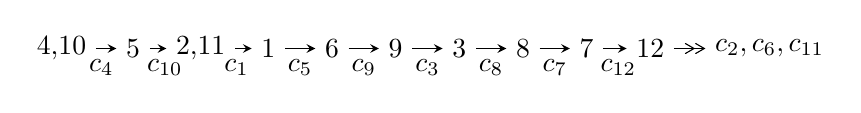
\begin{tikzpicture}[x=23pt, y=7pt]
	% node
	\node (A0) at (-1/8, 0) {4,10};
	\node (A1) at (1, 0) {5};
	\node (A2) at (33/16, 0) {2,11};
	\node (A3) at (25/8, 0) {1};
	\node (A4) at (33/8, 0) {6};
	\node (A5) at (41/8, 0) {9};
	\node (A6) at (49/8, 0) {3};
	\node (A7) at (57/8, 0) {8};
	\node (A8) at (65/8, 0) {7};
	\node (A9) at (73/8, 0) {12};
	\node (C1) at (1/2, -1) {$c_{4}$};
	\node (C2) at (3/2, -1) {$c_{10}$};
	\node (C3) at (21/8, -1) {$c_{1}$};
	\node (C4) at (29/8, -1) {$c_{5}$};
	\node (C5) at (37/8, -1) {$c_{9}$};
	\node (C6) at (45/8, -1) {$c_{3}$};
	\node (C7) at (53/8, -1) {$c_{8}$};
	\node (C8) at (61/8, -1) {$c_{7}$};
	\node (C9) at (69/8, -1) {$c_{12}$};
	\node (A10) at (11, 0) {$c_{2},c_{6},c_{11}$};

	% edge
	\draw[->,>=stealth]	
	(A0) edge (A1) (A1) edge (A2) (A2) edge (A3) (A3) edge (A4) (A4) edge (A5) (A5) edge (A6) (A6) edge (A7) (A7) edge (A8) (A8) edge (A9) ;
	\draw[->>,>={angle 60}]	
	(A9) edge (A10);
\end{tikzpicture} \\ 

\end{tabular} \\

\footnotetext{
The image of knot diagram is generated by the software ``\textbf{Draw programme}" developed by Andrew Bartholomew(\url{http://www.layer8.co.uk/maths/draw/index.htm\#Running-draw}), where we modified some parts for our purpose(\url{https://github.com/CATsTAILs/LinksPainter}).
}\phantom \\ \newline 
\centering \textbf{Ideals for irreducible components\footnotemark of $X_{\text{par}}$} 
 
\begin{align*}
I^u_{1}&=\langle 
3.85914\times10^{218} u^{85}+5.23238\times10^{218} u^{84}+\cdots+1.12919\times10^{219} b-4.30007\times10^{220},\\
\phantom{I^u_{1}}&\phantom{= \langle  }-5.00889\times10^{219} u^{85}-3.83512\times10^{219} u^{84}+\cdots+1.24211\times10^{220} a+1.01514\times10^{222},\\
\phantom{I^u_{1}}&\phantom{= \langle  }u^{86}-26 u^{84}+\cdots+352 u+143\rangle \\
I^u_{2}&=\langle 
-296859606 u^{23}-672784784 u^{22}+\cdots+1044681373 b-15785274596,\\
\phantom{I^u_{2}}&\phantom{= \langle  }642367601 u^{23}-9005160835 u^{22}+\cdots+9402132357 a+67337415889,\;u^{24}+u^{23}+\cdots+11 u+9\rangle \\
\\
\end{align*}
\raggedright * 2 irreducible components of $\dim_{\mathbb{C}}=0$, with total 110 representations.\\
\footnotetext{All coefficients of polynomials are rational numbers. But the coefficients are sometimes approximated in decimal forms when there is not enough margin.}
\newpage
\renewcommand{\arraystretch}{1}
\centering \section*{I. $I^u_{1}= \langle 3.86\times10^{218} u^{85}+5.23\times10^{218} u^{84}+\cdots+1.13\times10^{219} b-4.30\times10^{220},\;-5.01\times10^{219} u^{85}-3.84\times10^{219} u^{84}+\cdots+1.24\times10^{220} a+1.02\times10^{222},\;u^{86}-26 u^{84}+\cdots+352 u+143 \rangle$}
\flushleft \textbf{(i) Arc colorings}\\
\begin{tabular}{m{7pt} m{180pt} m{7pt} m{180pt} }
\flushright $a_{4}=$&$\begin{pmatrix}1\\0\end{pmatrix}$ \\
\flushright $a_{10}=$&$\begin{pmatrix}0\\u\end{pmatrix}$ \\
\flushright $a_{5}=$&$\begin{pmatrix}1\\u^2\end{pmatrix}$ \\
\flushright $a_{2}=$&$\begin{pmatrix}0.403257 u^{85}+0.308758 u^{84}+\cdots-295.596 u-81.7270\\-0.341761 u^{85}-0.463375 u^{84}+\cdots+115.690 u+38.0810\end{pmatrix}$ \\
\flushright $a_{11}=$&$\begin{pmatrix}- u\\- u^3+u\end{pmatrix}$ \\
\flushright $a_{1}=$&$\begin{pmatrix}0.0614956 u^{85}-0.154617 u^{84}+\cdots-179.905 u-43.6459\\-0.341761 u^{85}-0.463375 u^{84}+\cdots+115.690 u+38.0810\end{pmatrix}$ \\
\flushright $a_{6}=$&$\begin{pmatrix}3.44397 u^{85}+3.32938 u^{84}+\cdots-1720.90 u-500.050\\1.55973 u^{85}+1.31239 u^{84}+\cdots-940.484 u-263.433\end{pmatrix}$ \\
\flushright $a_{9}=$&$\begin{pmatrix}1.95617 u^{85}+2.18050 u^{84}+\cdots-673.241 u-213.966\\1.26891 u^{85}+1.09399 u^{84}+\cdots-711.937 u-198.806\end{pmatrix}$ \\
\flushright $a_{3}=$&$\begin{pmatrix}3.93599 u^{85}+3.76143 u^{84}+\cdots-1909.61 u-556.585\\-0.239645 u^{85}-0.0691656 u^{84}+\cdots+268.429 u+69.1359\end{pmatrix}$ \\
\flushright $a_{8}=$&$\begin{pmatrix}0.998356 u^{85}+1.19873 u^{84}+\cdots-230.274 u-83.7492\\1.25082 u^{85}+1.11752 u^{84}+\cdots-672.352 u-188.629\end{pmatrix}$ \\
\flushright $a_{7}=$&$\begin{pmatrix}1.64727 u^{85}+1.65507 u^{84}+\cdots-761.689 u-224.947\\1.85993 u^{85}+1.66888 u^{84}+\cdots-1053.41 u-299.108\end{pmatrix}$ \\
\flushright $a_{12}=$&$\begin{pmatrix}-1.44206 u^{85}+0.328546 u^{84}+\cdots+1873.41 u+470.130\\0.373170 u^{85}+0.655436 u^{84}+\cdots+29.6065 u-8.46160\end{pmatrix}$\\&\end{tabular}
\flushleft \textbf{(ii) Obstruction class $= -1$}\\~\\
\flushleft \textbf{(iii) Cusp Shapes $= -12.2613 u^{85}-19.5611 u^{84}+\cdots+770.668 u+597.207$}\\~\\
\newpage\renewcommand{\arraystretch}{1}
\flushleft \textbf{(iv) u-Polynomials at the component}\newline \\
\begin{tabular}{m{50pt}|m{274pt}}
Crossings & \hspace{64pt}u-Polynomials at each crossing \\
\hline $$\begin{aligned}c_{1}\end{aligned}$$&$\begin{aligned}
&u^{86}-3 u^{85}+\cdots-1090 u+331
\end{aligned}$\\
\hline $$\begin{aligned}c_{2},c_{7}\end{aligned}$$&$\begin{aligned}
&u^{86}+2 u^{85}+\cdots+98 u+47
\end{aligned}$\\
\hline $$\begin{aligned}c_{3}\end{aligned}$$&$\begin{aligned}
&u^{86}- u^{85}+\cdots-18 u+4
\end{aligned}$\\
\hline $$\begin{aligned}c_{4},c_{10}\end{aligned}$$&$\begin{aligned}
&u^{86}-26 u^{84}+\cdots-352 u+143
\end{aligned}$\\
\hline $$\begin{aligned}c_{5},c_{12}\end{aligned}$$&$\begin{aligned}
&u^{86}+u^{85}+\cdots-2490 u+2156
\end{aligned}$\\
\hline $$\begin{aligned}c_{6}\end{aligned}$$&$\begin{aligned}
&u^{86}-28 u^{84}+\cdots-145161863 u+33647749
\end{aligned}$\\
\hline $$\begin{aligned}c_{8},c_{11}\end{aligned}$$&$\begin{aligned}
&u^{86}+4 u^{85}+\cdots+460 u+221
\end{aligned}$\\
\hline $$\begin{aligned}c_{9}\end{aligned}$$&$\begin{aligned}
&u^{86}+2 u^{85}+\cdots+7484 u+1411
\end{aligned}$\\
\hline
\end{tabular}\\~\\
\newpage\renewcommand{\arraystretch}{1}
\flushleft \textbf{(v) Riley Polynomials at the component}\newline \\
\begin{tabular}{m{50pt}|m{274pt}}
Crossings & \hspace{64pt}Riley Polynomials at each crossing \\
\hline $$\begin{aligned}c_{1}\end{aligned}$$&$\begin{aligned}
&y^{86}-7 y^{85}+\cdots-234820 y+109561
\end{aligned}$\\
\hline $$\begin{aligned}c_{2},c_{7}\end{aligned}$$&$\begin{aligned}
&y^{86}-26 y^{85}+\cdots-35642 y+2209
\end{aligned}$\\
\hline $$\begin{aligned}c_{3}\end{aligned}$$&$\begin{aligned}
&y^{86}+31 y^{85}+\cdots-988 y+16
\end{aligned}$\\
\hline $$\begin{aligned}c_{4},c_{10}\end{aligned}$$&$\begin{aligned}
&y^{86}-52 y^{85}+\cdots-226292 y+20449
\end{aligned}$\\
\hline $$\begin{aligned}c_{5},c_{12}\end{aligned}$$&$\begin{aligned}
&y^{86}+59 y^{85}+\cdots+168629940 y+4648336
\end{aligned}$\\
\hline $$\begin{aligned}c_{6}\end{aligned}$$&$\begin{aligned}
&y^{86}-56 y^{85}+\cdots+41812736405652607 y+1132171012767001
\end{aligned}$\\
\hline $$\begin{aligned}c_{8},c_{11}\end{aligned}$$&$\begin{aligned}
&y^{86}+80 y^{85}+\cdots+18613622 y+48841
\end{aligned}$\\
\hline $$\begin{aligned}c_{9}\end{aligned}$$&$\begin{aligned}
&y^{86}+42 y^{85}+\cdots+83072014 y+1990921
\end{aligned}$\\
\hline
\end{tabular}\\~\\
\newpage\flushleft \textbf{(vi) Complex Volumes and Cusp Shapes}
$$\begin{array}{c|c|c}  
\text{Solutions to }I^u_{1}& \I (\text{vol} + \sqrt{-1}CS) & \text{Cusp shape}\\
 \hline 
\begin{aligned}
u &= \phantom{-}1.013240 + 0.156600 I \\
a &= \phantom{-}0.061933 - 0.617773 I \\
b &= -1.73273 + 2.09017 I\end{aligned}
 & -3.77856 - 6.86337 I & \phantom{-0.000000 } 0 \\ \hline\begin{aligned}
u &= \phantom{-}1.013240 - 0.156600 I \\
a &= \phantom{-}0.061933 + 0.617773 I \\
b &= -1.73273 - 2.09017 I\end{aligned}
 & -3.77856 + 6.86337 I & \phantom{-0.000000 } 0 \\ \hline\begin{aligned}
u &= \phantom{-}0.946501 + 0.164076 I \\
a &= \phantom{-}0.65342 + 2.54858 I \\
b &= \phantom{-}0.082485 - 0.387385 I\end{aligned}
 & -0.028740 - 0.605068 I & \phantom{-0.000000 } 0 \\ \hline\begin{aligned}
u &= \phantom{-}0.946501 - 0.164076 I \\
a &= \phantom{-}0.65342 - 2.54858 I \\
b &= \phantom{-}0.082485 + 0.387385 I\end{aligned}
 & -0.028740 + 0.605068 I & \phantom{-0.000000 } 0 \\ \hline\begin{aligned}
u &= \phantom{-}0.935366 + 0.122426 I \\
a &= \phantom{-}0.81877 + 1.57708 I \\
b &= \phantom{-}0.594883 - 0.656114 I\end{aligned}
 & \phantom{-}0.135026 - 0.962079 I & \phantom{-0.000000 } 0 \\ \hline\begin{aligned}
u &= \phantom{-}0.935366 - 0.122426 I \\
a &= \phantom{-}0.81877 - 1.57708 I \\
b &= \phantom{-}0.594883 + 0.656114 I\end{aligned}
 & \phantom{-}0.135026 + 0.962079 I & \phantom{-0.000000 } 0 \\ \hline\begin{aligned}
u &= -0.727128 + 0.584765 I \\
a &= -0.227558 + 1.248560 I \\
b &= \phantom{-}1.340550 - 0.264504 I\end{aligned}
 & -4.35117 - 0.02788 I & \phantom{-0.000000 } 0 \\ \hline\begin{aligned}
u &= -0.727128 - 0.584765 I \\
a &= -0.227558 - 1.248560 I \\
b &= \phantom{-}1.340550 + 0.264504 I\end{aligned}
 & -4.35117 + 0.02788 I & \phantom{-0.000000 } 0 \\ \hline\begin{aligned}
u &= -0.924847 + 0.536642 I \\
a &= -0.347462 + 0.979449 I \\
b &= \phantom{-}0.054894 - 0.770968 I\end{aligned}
 & \phantom{-}1.42029 + 4.02474 I & \phantom{-0.000000 } 0 \\ \hline\begin{aligned}
u &= -0.924847 - 0.536642 I \\
a &= -0.347462 - 0.979449 I \\
b &= \phantom{-}0.054894 + 0.770968 I\end{aligned}
 & \phantom{-}1.42029 - 4.02474 I & \phantom{-0.000000 } 0\\
 \hline 
 \end{array}$$\newpage$$\begin{array}{c|c|c}  
\text{Solutions to }I^u_{1}& \I (\text{vol} + \sqrt{-1}CS) & \text{Cusp shape}\\
 \hline 
\begin{aligned}
u &= \phantom{-}1.019770 + 0.327343 I \\
a &= -1.53537 + 0.31678 I \\
b &= -0.358846 - 0.491803 I\end{aligned}
 & -3.49969 - 2.27160 I & \phantom{-0.000000 } 0 \\ \hline\begin{aligned}
u &= \phantom{-}1.019770 - 0.327343 I \\
a &= -1.53537 - 0.31678 I \\
b &= -0.358846 + 0.491803 I\end{aligned}
 & -3.49969 + 2.27160 I & \phantom{-0.000000 } 0 \\ \hline\begin{aligned}
u &= -1.001200 + 0.393657 I \\
a &= \phantom{-}1.62994 + 0.27952 I \\
b &= \phantom{-}0.449265 - 0.605829 I\end{aligned}
 & -2.03015 + 9.00043 I & \phantom{-0.000000 } 0 \\ \hline\begin{aligned}
u &= -1.001200 - 0.393657 I \\
a &= \phantom{-}1.62994 - 0.27952 I \\
b &= \phantom{-}0.449265 + 0.605829 I\end{aligned}
 & -2.03015 - 9.00043 I & \phantom{-0.000000 } 0 \\ \hline\begin{aligned}
u &= -1.075550 + 0.027859 I \\
a &= \phantom{-}0.168250 - 0.671082 I \\
b &= \phantom{-}1.99103 + 1.12349 I\end{aligned}
 & -6.51206 - 0.43126 I & \phantom{-0.000000 } 0 \\ \hline\begin{aligned}
u &= -1.075550 - 0.027859 I \\
a &= \phantom{-}0.168250 + 0.671082 I \\
b &= \phantom{-}1.99103 - 1.12349 I\end{aligned}
 & -6.51206 + 0.43126 I & \phantom{-0.000000 } 0 \\ \hline\begin{aligned}
u &= \phantom{-}0.899199 + 0.142670 I \\
a &= \phantom{-}0.61730 + 1.32859 I \\
b &= \phantom{-}0.657270 - 0.389408 I\end{aligned}
 & \phantom{-}0.165768 - 0.366994 I & \phantom{-0.000000 } 0 \\ \hline\begin{aligned}
u &= \phantom{-}0.899199 - 0.142670 I \\
a &= \phantom{-}0.61730 - 1.32859 I \\
b &= \phantom{-}0.657270 + 0.389408 I\end{aligned}
 & \phantom{-}0.165768 + 0.366994 I & \phantom{-0.000000 } 0 \\ \hline\begin{aligned}
u &= -0.015482 + 1.089660 I \\
a &= -0.915625 - 0.620168 I \\
b &= \phantom{-}0.775767 + 0.822352 I\end{aligned}
 & -2.38759 - 4.54755 I & \phantom{-0.000000 } 0 \\ \hline\begin{aligned}
u &= -0.015482 - 1.089660 I \\
a &= -0.915625 + 0.620168 I \\
b &= \phantom{-}0.775767 - 0.822352 I\end{aligned}
 & -2.38759 + 4.54755 I & \phantom{-0.000000 } 0\\
 \hline 
 \end{array}$$\newpage$$\begin{array}{c|c|c}  
\text{Solutions to }I^u_{1}& \I (\text{vol} + \sqrt{-1}CS) & \text{Cusp shape}\\
 \hline 
\begin{aligned}
u &= -0.455919 + 0.998858 I \\
a &= \phantom{-}0.337485 + 0.103051 I \\
b &= -0.571382 - 0.676993 I\end{aligned}
 & \phantom{-}4.83318 + 0.07837 I & \phantom{-0.000000 } 0 \\ \hline\begin{aligned}
u &= -0.455919 - 0.998858 I \\
a &= \phantom{-}0.337485 - 0.103051 I \\
b &= -0.571382 + 0.676993 I\end{aligned}
 & \phantom{-}4.83318 - 0.07837 I & \phantom{-0.000000 } 0 \\ \hline\begin{aligned}
u &= -1.069760 + 0.330003 I \\
a &= -0.395329 + 0.520215 I \\
b &= -0.654977 - 0.341910 I\end{aligned}
 & \phantom{-}1.07982 + 3.82086 I & \phantom{-0.000000 } 0 \\ \hline\begin{aligned}
u &= -1.069760 - 0.330003 I \\
a &= -0.395329 - 0.520215 I \\
b &= -0.654977 + 0.341910 I\end{aligned}
 & \phantom{-}1.07982 - 3.82086 I & \phantom{-0.000000 } 0 \\ \hline\begin{aligned}
u &= \phantom{-}0.279630 + 0.827400 I \\
a &= \phantom{-}0.723072 + 1.097880 I \\
b &= -1.033860 - 0.336513 I\end{aligned}
 & -4.18891 - 5.58599 I & \phantom{-0.000000 } 0 \\ \hline\begin{aligned}
u &= \phantom{-}0.279630 - 0.827400 I \\
a &= \phantom{-}0.723072 - 1.097880 I \\
b &= -1.033860 + 0.336513 I\end{aligned}
 & -4.18891 + 5.58599 I & \phantom{-0.000000 } 0 \\ \hline\begin{aligned}
u &= -0.862909 + 0.134585 I \\
a &= -0.72937 - 1.80432 I \\
b &= -0.642795 + 1.145470 I\end{aligned}
 & \phantom{-}3.92961 + 2.85500 I & \phantom{-0.000000 } 0 \\ \hline\begin{aligned}
u &= -0.862909 - 0.134585 I \\
a &= -0.72937 + 1.80432 I \\
b &= -0.642795 - 1.145470 I\end{aligned}
 & \phantom{-}3.92961 - 2.85500 I & \phantom{-0.000000 } 0 \\ \hline\begin{aligned}
u &= -0.782385 + 0.368272 I \\
a &= \phantom{-}1.43549 - 0.13900 I \\
b &= -0.314156 - 0.491568 I\end{aligned}
 & \phantom{-}3.63471 - 0.52145 I & \phantom{-0.000000 } 0 \\ \hline\begin{aligned}
u &= -0.782385 - 0.368272 I \\
a &= \phantom{-}1.43549 + 0.13900 I \\
b &= -0.314156 + 0.491568 I\end{aligned}
 & \phantom{-}3.63471 + 0.52145 I & \phantom{-0.000000 } 0\\
 \hline 
 \end{array}$$\newpage$$\begin{array}{c|c|c}  
\text{Solutions to }I^u_{1}& \I (\text{vol} + \sqrt{-1}CS) & \text{Cusp shape}\\
 \hline 
\begin{aligned}
u &= -0.014150 + 1.172740 I \\
a &= -0.544027 + 0.153648 I \\
b &= \phantom{-}0.320054 - 0.610257 I\end{aligned}
 & \phantom{-}4.62544 + 0.94388 I & \phantom{-0.000000 } 0 \\ \hline\begin{aligned}
u &= -0.014150 - 1.172740 I \\
a &= -0.544027 - 0.153648 I \\
b &= \phantom{-}0.320054 + 0.610257 I\end{aligned}
 & \phantom{-}4.62544 - 0.94388 I & \phantom{-0.000000 } 0 \\ \hline\begin{aligned}
u &= \phantom{-}0.140588 + 1.189710 I \\
a &= \phantom{-}0.908141 - 0.496246 I \\
b &= -0.831187 + 0.816196 I\end{aligned}
 & -1.25558 + 11.17520 I & \phantom{-0.000000 } 0 \\ \hline\begin{aligned}
u &= \phantom{-}0.140588 - 1.189710 I \\
a &= \phantom{-}0.908141 + 0.496246 I \\
b &= -0.831187 - 0.816196 I\end{aligned}
 & -1.25558 - 11.17520 I & \phantom{-0.000000 } 0 \\ \hline\begin{aligned}
u &= -0.359459 + 1.155750 I \\
a &= \phantom{-}0.585216 + 0.275949 I \\
b &= -0.633762 - 0.485525 I\end{aligned}
 & \phantom{-}3.14464 - 2.91301 I & \phantom{-0.000000 } 0 \\ \hline\begin{aligned}
u &= -0.359459 - 1.155750 I \\
a &= \phantom{-}0.585216 - 0.275949 I \\
b &= -0.633762 + 0.485525 I\end{aligned}
 & \phantom{-}3.14464 + 2.91301 I & \phantom{-0.000000 } 0 \\ \hline\begin{aligned}
u &= \phantom{-}0.741114 + 0.128033 I \\
a &= -1.219120 - 0.690485 I \\
b &= -1.57726 - 0.48897 I\end{aligned}
 & -2.91270 + 5.35630 I & \phantom{-}0.19430 - 2.58314 I \\ \hline\begin{aligned}
u &= \phantom{-}0.741114 - 0.128033 I \\
a &= -1.219120 + 0.690485 I \\
b &= -1.57726 + 0.48897 I\end{aligned}
 & -2.91270 - 5.35630 I & \phantom{-}0.19430 + 2.58314 I \\ \hline\begin{aligned}
u &= \phantom{-}1.224260 + 0.308586 I \\
a &= \phantom{-}0.37545 - 1.41933 I \\
b &= \phantom{-}1.007880 + 0.816912 I\end{aligned}
 & -8.64326 - 2.65098 I & \phantom{-0.000000 } 0 \\ \hline\begin{aligned}
u &= \phantom{-}1.224260 - 0.308586 I \\
a &= \phantom{-}0.37545 + 1.41933 I \\
b &= \phantom{-}1.007880 - 0.816912 I\end{aligned}
 & -8.64326 + 2.65098 I & \phantom{-0.000000 } 0\\
 \hline 
 \end{array}$$\newpage$$\begin{array}{c|c|c}  
\text{Solutions to }I^u_{1}& \I (\text{vol} + \sqrt{-1}CS) & \text{Cusp shape}\\
 \hline 
\begin{aligned}
u &= \phantom{-}1.243050 + 0.241448 I \\
a &= -0.357460 + 0.539477 I \\
b &= -0.790416 - 0.344192 I\end{aligned}
 & -2.99529 - 0.68487 I & \phantom{-0.000000 } 0 \\ \hline\begin{aligned}
u &= \phantom{-}1.243050 - 0.241448 I \\
a &= -0.357460 - 0.539477 I \\
b &= -0.790416 + 0.344192 I\end{aligned}
 & -2.99529 + 0.68487 I & \phantom{-0.000000 } 0 \\ \hline\begin{aligned}
u &= \phantom{-}1.194790 + 0.422230 I \\
a &= -0.463621 + 0.994886 I \\
b &= -1.26517 - 1.42297 I\end{aligned}
 & \phantom{-}2.82983 - 6.91529 I & \phantom{-0.000000 } 0 \\ \hline\begin{aligned}
u &= \phantom{-}1.194790 - 0.422230 I \\
a &= -0.463621 - 0.994886 I \\
b &= -1.26517 + 1.42297 I\end{aligned}
 & \phantom{-}2.82983 + 6.91529 I & \phantom{-0.000000 } 0 \\ \hline\begin{aligned}
u &= -1.245920 + 0.275497 I \\
a &= \phantom{-}0.260591 + 0.811687 I \\
b &= \phantom{-}0.999528 - 0.947180 I\end{aligned}
 & -4.17702 + 3.64369 I & \phantom{-0.000000 } 0 \\ \hline\begin{aligned}
u &= -1.245920 - 0.275497 I \\
a &= \phantom{-}0.260591 - 0.811687 I \\
b &= \phantom{-}0.999528 + 0.947180 I\end{aligned}
 & -4.17702 - 3.64369 I & \phantom{-0.000000 } 0 \\ \hline\begin{aligned}
u &= -1.177240 + 0.541228 I \\
a &= -0.278209 - 0.658710 I \\
b &= -1.31264 + 0.74781 I\end{aligned}
 & \phantom{-}2.32587 + 5.43706 I & \phantom{-0.000000 } 0 \\ \hline\begin{aligned}
u &= -1.177240 - 0.541228 I \\
a &= -0.278209 + 0.658710 I \\
b &= -1.31264 - 0.74781 I\end{aligned}
 & \phantom{-}2.32587 - 5.43706 I & \phantom{-0.000000 } 0 \\ \hline\begin{aligned}
u &= \phantom{-}0.225617 + 0.639859 I \\
a &= \phantom{-}1.48458 - 0.79709 I \\
b &= -0.584963 + 1.170950 I\end{aligned}
 & \phantom{-}5.82789 + 2.77163 I & \phantom{-}3.62621 - 5.12009 I \\ \hline\begin{aligned}
u &= \phantom{-}0.225617 - 0.639859 I \\
a &= \phantom{-}1.48458 + 0.79709 I \\
b &= -0.584963 - 1.170950 I\end{aligned}
 & \phantom{-}5.82789 - 2.77163 I & \phantom{-}3.62621 + 5.12009 I\\
 \hline 
 \end{array}$$\newpage$$\begin{array}{c|c|c}  
\text{Solutions to }I^u_{1}& \I (\text{vol} + \sqrt{-1}CS) & \text{Cusp shape}\\
 \hline 
\begin{aligned}
u &= -1.320110 + 0.173352 I \\
a &= \phantom{-}0.192094 + 0.541101 I \\
b &= \phantom{-}0.00408 - 1.94041 I\end{aligned}
 & -5.93895 + 3.63950 I & \phantom{-0.000000 } 0 \\ \hline\begin{aligned}
u &= -1.320110 - 0.173352 I \\
a &= \phantom{-}0.192094 - 0.541101 I \\
b &= \phantom{-}0.00408 + 1.94041 I\end{aligned}
 & -5.93895 - 3.63950 I & \phantom{-0.000000 } 0 \\ \hline\begin{aligned}
u &= -0.397923 + 0.534043 I \\
a &= \phantom{-}0.09432 - 1.75717 I \\
b &= \phantom{-}0.309084 + 1.191700 I\end{aligned}
 & -0.33732 - 5.25732 I & \phantom{-}3.19134 + 2.30399 I \\ \hline\begin{aligned}
u &= -0.397923 - 0.534043 I \\
a &= \phantom{-}0.09432 + 1.75717 I \\
b &= \phantom{-}0.309084 - 1.191700 I\end{aligned}
 & -0.33732 + 5.25732 I & \phantom{-}3.19134 - 2.30399 I \\ \hline\begin{aligned}
u &= -1.281140 + 0.379028 I \\
a &= -0.344880 - 1.318420 I \\
b &= -1.022710 + 0.788679 I\end{aligned}
 & -8.77560 + 9.65768 I & \phantom{-0.000000 } 0 \\ \hline\begin{aligned}
u &= -1.281140 - 0.379028 I \\
a &= -0.344880 + 1.318420 I \\
b &= -1.022710 - 0.788679 I\end{aligned}
 & -8.77560 - 9.65768 I & \phantom{-0.000000 } 0 \\ \hline\begin{aligned}
u &= \phantom{-}1.348360 + 0.054033 I \\
a &= -0.061038 - 0.473724 I \\
b &= \phantom{-}0.93523 + 2.02994 I\end{aligned}
 & -6.00193 - 4.32624 I & \phantom{-0.000000 } 0 \\ \hline\begin{aligned}
u &= \phantom{-}1.348360 - 0.054033 I \\
a &= -0.061038 + 0.473724 I \\
b &= \phantom{-}0.93523 - 2.02994 I\end{aligned}
 & -6.00193 + 4.32624 I & \phantom{-0.000000 } 0 \\ \hline\begin{aligned}
u &= \phantom{-}0.463929 + 1.273310 I \\
a &= -0.566675 + 0.091422 I \\
b &= \phantom{-}0.488847 - 0.410672 I\end{aligned}
 & \phantom{-}2.63674 - 1.06753 I & \phantom{-0.000000 } 0 \\ \hline\begin{aligned}
u &= \phantom{-}0.463929 - 1.273310 I \\
a &= -0.566675 - 0.091422 I \\
b &= \phantom{-}0.488847 + 0.410672 I\end{aligned}
 & \phantom{-}2.63674 + 1.06753 I & \phantom{-0.000000 } 0\\
 \hline 
 \end{array}$$\newpage$$\begin{array}{c|c|c}  
\text{Solutions to }I^u_{1}& \I (\text{vol} + \sqrt{-1}CS) & \text{Cusp shape}\\
 \hline 
\begin{aligned}
u &= -1.148330 + 0.759634 I \\
a &= -0.459012 + 0.592200 I \\
b &= \phantom{-}1.317320 + 0.103020 I\end{aligned}
 & -5.56625 + 5.77682 I & \phantom{-0.000000 } 0 \\ \hline\begin{aligned}
u &= -1.148330 - 0.759634 I \\
a &= -0.459012 - 0.592200 I \\
b &= \phantom{-}1.317320 - 0.103020 I\end{aligned}
 & -5.56625 - 5.77682 I & \phantom{-0.000000 } 0 \\ \hline\begin{aligned}
u &= \phantom{-}0.203161 + 0.556123 I \\
a &= -0.48221 - 1.79807 I \\
b &= -0.262667 + 1.008830 I\end{aligned}
 & -1.28788 - 1.11969 I & \phantom{-}2.17883 + 1.74771 I \\ \hline\begin{aligned}
u &= \phantom{-}0.203161 - 0.556123 I \\
a &= -0.48221 + 1.79807 I \\
b &= -0.262667 - 1.008830 I\end{aligned}
 & -1.28788 + 1.11969 I & \phantom{-}2.17883 - 1.74771 I \\ \hline\begin{aligned}
u &= -0.454810 + 0.375338 I \\
a &= -1.59503 - 0.91449 I \\
b &= -0.496780 + 0.231794 I\end{aligned}
 & \phantom{-}2.81852 - 0.19677 I & \phantom{-}3.08966 - 3.01616 I \\ \hline\begin{aligned}
u &= -0.454810 - 0.375338 I \\
a &= -1.59503 + 0.91449 I \\
b &= -0.496780 - 0.231794 I\end{aligned}
 & \phantom{-}2.81852 + 0.19677 I & \phantom{-}3.08966 + 3.01616 I \\ \hline\begin{aligned}
u &= \phantom{-}1.25089 + 0.68548 I \\
a &= \phantom{-}0.006593 - 0.938843 I \\
b &= \phantom{-}1.023550 + 0.815519 I\end{aligned}
 & -0.12254 - 5.71927 I & \phantom{-0.000000 } 0 \\ \hline\begin{aligned}
u &= \phantom{-}1.25089 - 0.68548 I \\
a &= \phantom{-}0.006593 + 0.938843 I \\
b &= \phantom{-}1.023550 - 0.815519 I\end{aligned}
 & -0.12254 + 5.71927 I & \phantom{-0.000000 } 0 \\ \hline\begin{aligned}
u &= -1.28080 + 0.63183 I \\
a &= -0.220888 - 0.959005 I \\
b &= -1.077160 + 0.774774 I\end{aligned}
 & \phantom{-}0.04388 + 9.24471 I & \phantom{-0.000000 } 0 \\ \hline\begin{aligned}
u &= -1.28080 - 0.63183 I \\
a &= -0.220888 + 0.959005 I \\
b &= -1.077160 - 0.774774 I\end{aligned}
 & \phantom{-}0.04388 - 9.24471 I & \phantom{-0.000000 } 0\\
 \hline 
 \end{array}$$\newpage$$\begin{array}{c|c|c}  
\text{Solutions to }I^u_{1}& \I (\text{vol} + \sqrt{-1}CS) & \text{Cusp shape}\\
 \hline 
\begin{aligned}
u &= \phantom{-}1.28042 + 0.65504 I \\
a &= \phantom{-}0.265807 + 0.510700 I \\
b &= -1.178570 + 0.010457 I\end{aligned}
 & -6.88725 - 0.19421 I & \phantom{-0.000000 } 0 \\ \hline\begin{aligned}
u &= \phantom{-}1.28042 - 0.65504 I \\
a &= \phantom{-}0.265807 - 0.510700 I \\
b &= -1.178570 - 0.010457 I\end{aligned}
 & -6.88725 + 0.19421 I & \phantom{-0.000000 } 0 \\ \hline\begin{aligned}
u &= -1.34096 + 0.53769 I \\
a &= \phantom{-}0.213817 + 1.052190 I \\
b &= \phantom{-}1.32707 - 1.16128 I\end{aligned}
 & -6.52492 + 10.27030 I & \phantom{-0.000000 } 0 \\ \hline\begin{aligned}
u &= -1.34096 - 0.53769 I \\
a &= \phantom{-}0.213817 - 1.052190 I \\
b &= \phantom{-}1.32707 + 1.16128 I\end{aligned}
 & -6.52492 - 10.27030 I & \phantom{-0.000000 } 0 \\ \hline\begin{aligned}
u &= \phantom{-}1.34112 + 0.60712 I \\
a &= -0.166632 + 1.083530 I \\
b &= -1.36056 - 1.11761 I\end{aligned}
 & -5.0587 - 17.4655 I & \phantom{-0.000000 } 0 \\ \hline\begin{aligned}
u &= \phantom{-}1.34112 - 0.60712 I \\
a &= -0.166632 - 1.083530 I \\
b &= -1.36056 + 1.11761 I\end{aligned}
 & -5.0587 + 17.4655 I & \phantom{-0.000000 } 0 \\ \hline\begin{aligned}
u &= \phantom{-}1.40203 + 0.59947 I \\
a &= \phantom{-}0.034030 - 0.722008 I \\
b &= \phantom{-}1.06930 + 0.97248 I\end{aligned}
 & \phantom{-}0.13038 - 7.25479 I & \phantom{-0.000000 } 0 \\ \hline\begin{aligned}
u &= \phantom{-}1.40203 - 0.59947 I \\
a &= \phantom{-}0.034030 + 0.722008 I \\
b &= \phantom{-}1.06930 - 0.97248 I\end{aligned}
 & \phantom{-}0.13038 + 7.25479 I & \phantom{-0.000000 } 0 \\ \hline\begin{aligned}
u &= \phantom{-}1.45765 + 0.48227 I \\
a &= -0.317056 - 0.548033 I \\
b &= \phantom{-}0.568832 + 0.060403 I\end{aligned}
 & -7.04915 - 1.30997 I & \phantom{-0.000000 } 0 \\ \hline\begin{aligned}
u &= \phantom{-}1.45765 - 0.48227 I \\
a &= -0.317056 + 0.548033 I \\
b &= \phantom{-}0.568832 - 0.060403 I\end{aligned}
 & -7.04915 + 1.30997 I & \phantom{-0.000000 } 0\\
 \hline 
 \end{array}$$\newpage$$\begin{array}{c|c|c}  
\text{Solutions to }I^u_{1}& \I (\text{vol} + \sqrt{-1}CS) & \text{Cusp shape}\\
 \hline 
\begin{aligned}
u &= \phantom{-}0.175247 + 0.400925 I \\
a &= -0.777483 - 1.083630 I \\
b &= \phantom{-}0.313669 + 0.457730 I\end{aligned}
 & -0.028154 - 1.020300 I & -0.58024 + 6.60259 I \\ \hline\begin{aligned}
u &= \phantom{-}0.175247 - 0.400925 I \\
a &= -0.777483 + 1.083630 I \\
b &= \phantom{-}0.313669 - 0.457730 I\end{aligned}
 & -0.028154 + 1.020300 I & -0.58024 - 6.60259 I \\ \hline\begin{aligned}
u &= -0.285471 + 0.308360 I \\
a &= -0.68087 + 2.61679 I \\
b &= \phantom{-}1.111320 - 0.014505 I\end{aligned}
 & -4.45448 - 0.17557 I & -1.85939 + 1.38698 I \\ \hline\begin{aligned}
u &= -0.285471 - 0.308360 I \\
a &= -0.68087 - 2.61679 I \\
b &= \phantom{-}1.111320 + 0.014505 I\end{aligned}
 & -4.45448 + 0.17557 I & -1.85939 - 1.38698 I \\ \hline\begin{aligned}
u &= -1.56445 + 0.30136 I \\
a &= \phantom{-}0.203232 - 0.547484 I \\
b &= -0.539303 + 0.124283 I\end{aligned}
 & -7.16487 - 5.31827 I & \phantom{-0.000000 } 0 \\ \hline\begin{aligned}
u &= -1.56445 - 0.30136 I \\
a &= \phantom{-}0.203232 + 0.547484 I \\
b &= -0.539303 - 0.124283 I\end{aligned}
 & -7.16487 + 5.31827 I & \phantom{-0.000000 } 0\\
 \hline 
 \end{array}$$\newpage\newpage\renewcommand{\arraystretch}{1}
\centering \section*{II. $I^u_{2}= \langle -2.97\times10^{8} u^{23}-6.73\times10^{8} u^{22}+\cdots+1.04\times10^{9} b-1.58\times10^{10},\;6.42\times10^{8} u^{23}-9.01\times10^{9} u^{22}+\cdots+9.40\times10^{9} a+6.73\times10^{10},\;u^{24}+u^{23}+\cdots+11 u+9 \rangle$}
\flushleft \textbf{(i) Arc colorings}\\
\begin{tabular}{m{7pt} m{180pt} m{7pt} m{180pt} }
\flushright $a_{4}=$&$\begin{pmatrix}1\\0\end{pmatrix}$ \\
\flushright $a_{10}=$&$\begin{pmatrix}0\\u\end{pmatrix}$ \\
\flushright $a_{5}=$&$\begin{pmatrix}1\\u^2\end{pmatrix}$ \\
\flushright $a_{2}=$&$\begin{pmatrix}-0.0683215 u^{23}+0.957779 u^{22}+\cdots-12.5163 u-7.16193\\0.284163 u^{23}+0.644010 u^{22}+\cdots-4.87488 u+15.1101\end{pmatrix}$ \\
\flushright $a_{11}=$&$\begin{pmatrix}- u\\- u^3+u\end{pmatrix}$ \\
\flushright $a_{1}=$&$\begin{pmatrix}0.215841 u^{23}+1.60179 u^{22}+\cdots-17.3912 u+7.94820\\0.284163 u^{23}+0.644010 u^{22}+\cdots-4.87488 u+15.1101\end{pmatrix}$ \\
\flushright $a_{6}=$&$\begin{pmatrix}3.23542 u^{23}-1.25211 u^{22}+\cdots+40.0876 u+50.1277\\1.02610 u^{23}+0.164052 u^{22}+\cdots+4.58961 u+8.61489\end{pmatrix}$ \\
\flushright $a_{9}=$&$\begin{pmatrix}-3.26278 u^{23}-2.30081 u^{22}+\cdots+25.5811 u-8.57595\\2.43206 u^{23}+0.487842 u^{22}+\cdots+3.07086 u+28.7240\end{pmatrix}$ \\
\flushright $a_{3}=$&$\begin{pmatrix}-3.25988 u^{23}-0.801721 u^{22}+\cdots-7.72825 u-31.1982\\2.75440 u^{23}-0.528177 u^{22}+\cdots+19.1185 u+17.5731\end{pmatrix}$ \\
\flushright $a_{8}=$&$\begin{pmatrix}-3.09380 u^{23}-1.76139 u^{22}+\cdots+19.0783 u-24.4526\\3.53147 u^{23}+0.759929 u^{22}+\cdots+3.97813 u+41.2668\end{pmatrix}$ \\
\flushright $a_{7}=$&$\begin{pmatrix}1.18809 u^{23}-0.634541 u^{22}+\cdots+21.0603 u+21.8155\\1.76957 u^{23}-0.340698 u^{22}+\cdots+12.7290 u+12.9430\end{pmatrix}$ \\
\flushright $a_{12}=$&$\begin{pmatrix}-7.44088 u^{23}-7.91373 u^{22}+\cdots+54.5822 u+4.86864\\-1.49142 u^{23}-0.0977790 u^{22}+\cdots-5.81025 u-11.7070\end{pmatrix}$\\&\end{tabular}
\flushleft \textbf{(ii) Obstruction class $= 1$}\\~\\
\flushleft \textbf{(iii) Cusp Shapes $= -\frac{19642376118}{1044681373} u^{23}-\frac{39745603928}{1044681373} u^{22}+\cdots+\frac{416986178422}{1044681373} u+\frac{161826406806}{1044681373}$}\\~\\
\newpage\renewcommand{\arraystretch}{1}
\flushleft \textbf{(iv) u-Polynomials at the component}\newline \\
\begin{tabular}{m{50pt}|m{274pt}}
Crossings & \hspace{64pt}u-Polynomials at each crossing \\
\hline $$\begin{aligned}c_{1}\end{aligned}$$&$\begin{aligned}
&u^{24}+2 u^{22}+\cdots-3 u+1
\end{aligned}$\\
\hline $$\begin{aligned}c_{2}\end{aligned}$$&$\begin{aligned}
&u^{24}+u^{23}+\cdots+u+1
\end{aligned}$\\
\hline $$\begin{aligned}c_{3}\end{aligned}$$&$\begin{aligned}
&u^{24}+3 u^{22}+\cdots+101 u+11
\end{aligned}$\\
\hline $$\begin{aligned}c_{4}\end{aligned}$$&$\begin{aligned}
&u^{24}+u^{23}+\cdots+11 u+9
\end{aligned}$\\
\hline $$\begin{aligned}c_{5}\end{aligned}$$&$\begin{aligned}
&u^{24}+17 u^{22}+\cdots-2 u+5
\end{aligned}$\\
\hline $$\begin{aligned}c_{6}\end{aligned}$$&$\begin{aligned}
&u^{24}- u^{23}+\cdots-10 u+1
\end{aligned}$\\
\hline $$\begin{aligned}c_{7}\end{aligned}$$&$\begin{aligned}
&u^{24}- u^{23}+\cdots- u+1
\end{aligned}$\\
\hline $$\begin{aligned}c_{8}\end{aligned}$$&$\begin{aligned}
&u^{24}+u^{23}+\cdots+u+1
\end{aligned}$\\
\hline $$\begin{aligned}c_{9}\end{aligned}$$&$\begin{aligned}
&u^{24}+u^{23}+\cdots+u+1
\end{aligned}$\\
\hline $$\begin{aligned}c_{10}\end{aligned}$$&$\begin{aligned}
&u^{24}- u^{23}+\cdots-11 u+9
\end{aligned}$\\
\hline $$\begin{aligned}c_{11}\end{aligned}$$&$\begin{aligned}
&u^{24}- u^{23}+\cdots- u+1
\end{aligned}$\\
\hline $$\begin{aligned}c_{12}\end{aligned}$$&$\begin{aligned}
&u^{24}+17 u^{22}+\cdots+2 u+5
\end{aligned}$\\
\hline
\end{tabular}\\~\\
\newpage\renewcommand{\arraystretch}{1}
\flushleft \textbf{(v) Riley Polynomials at the component}\newline \\
\begin{tabular}{m{50pt}|m{274pt}}
Crossings & \hspace{64pt}Riley Polynomials at each crossing \\
\hline $$\begin{aligned}c_{1}\end{aligned}$$&$\begin{aligned}
&y^{24}+4 y^{23}+\cdots+21 y+1
\end{aligned}$\\
\hline $$\begin{aligned}c_{2},c_{7}\end{aligned}$$&$\begin{aligned}
&y^{24}-15 y^{23}+\cdots-9 y+1
\end{aligned}$\\
\hline $$\begin{aligned}c_{3}\end{aligned}$$&$\begin{aligned}
&y^{24}+6 y^{23}+\cdots-1577 y+121
\end{aligned}$\\
\hline $$\begin{aligned}c_{4},c_{10}\end{aligned}$$&$\begin{aligned}
&y^{24}-13 y^{23}+\cdots-679 y+81
\end{aligned}$\\
\hline $$\begin{aligned}c_{5},c_{12}\end{aligned}$$&$\begin{aligned}
&y^{24}+34 y^{23}+\cdots+446 y+25
\end{aligned}$\\
\hline $$\begin{aligned}c_{6}\end{aligned}$$&$\begin{aligned}
&y^{24}+3 y^{23}+\cdots+180 y+1
\end{aligned}$\\
\hline $$\begin{aligned}c_{8},c_{11}\end{aligned}$$&$\begin{aligned}
&y^{24}+19 y^{23}+\cdots-13 y+1
\end{aligned}$\\
\hline $$\begin{aligned}c_{9}\end{aligned}$$&$\begin{aligned}
&y^{24}+21 y^{23}+\cdots+11 y+1
\end{aligned}$\\
\hline
\end{tabular}\\~\\
\newpage\flushleft \textbf{(vi) Complex Volumes and Cusp Shapes}
$$\begin{array}{c|c|c}  
\text{Solutions to }I^u_{2}& \I (\text{vol} + \sqrt{-1}CS) & \text{Cusp shape}\\
 \hline 
\begin{aligned}
u &= \phantom{-}0.952348 + 0.136908 I \\
a &= \phantom{-}0.72993 + 2.89697 I \\
b &= \phantom{-}0.131126 - 0.384738 I\end{aligned}
 & -0.000597 - 0.548184 I & \phantom{-}24.3042 - 84.4549 I \\ \hline\begin{aligned}
u &= \phantom{-}0.952348 - 0.136908 I \\
a &= \phantom{-}0.72993 - 2.89697 I \\
b &= \phantom{-}0.131126 + 0.384738 I\end{aligned}
 & -0.000597 + 0.548184 I & \phantom{-}24.3042 + 84.4549 I \\ \hline\begin{aligned}
u &= \phantom{-}0.988311 + 0.370395 I \\
a &= -0.337958 + 0.880219 I \\
b &= -1.277510 + 0.015717 I\end{aligned}
 & -5.14631 - 0.87736 I & -4.28774 + 2.87316 I \\ \hline\begin{aligned}
u &= \phantom{-}0.988311 - 0.370395 I \\
a &= -0.337958 - 0.880219 I \\
b &= -1.277510 - 0.015717 I\end{aligned}
 & -5.14631 + 0.87736 I & -4.28774 - 2.87316 I \\ \hline\begin{aligned}
u &= \phantom{-}0.219364 + 1.039820 I \\
a &= \phantom{-}0.392367 - 0.200232 I \\
b &= -0.221572 - 0.274980 I\end{aligned}
 & \phantom{-}2.62740 - 1.82881 I & \phantom{-}0.54296 + 5.92489 I \\ \hline\begin{aligned}
u &= \phantom{-}0.219364 - 1.039820 I \\
a &= \phantom{-}0.392367 + 0.200232 I \\
b &= -0.221572 + 0.274980 I\end{aligned}
 & \phantom{-}2.62740 + 1.82881 I & \phantom{-}0.54296 - 5.92489 I \\ \hline\begin{aligned}
u &= -0.898687 + 0.258451 I \\
a &= \phantom{-}0.41561 + 1.84019 I \\
b &= \phantom{-}0.391206 - 1.205940 I\end{aligned}
 & \phantom{-}3.96928 + 3.45621 I & \phantom{-}4.14366 - 9.44746 I \\ \hline\begin{aligned}
u &= -0.898687 - 0.258451 I \\
a &= \phantom{-}0.41561 - 1.84019 I \\
b &= \phantom{-}0.391206 + 1.205940 I\end{aligned}
 & \phantom{-}3.96928 - 3.45621 I & \phantom{-}4.14366 + 9.44746 I \\ \hline\begin{aligned}
u &= \phantom{-}0.429227 + 0.822759 I \\
a &= -0.974193 + 0.323868 I \\
b &= \phantom{-}0.705339 - 1.048650 I\end{aligned}
 & \phantom{-}6.57769 + 1.81596 I & \phantom{-}7.75965 - 0.93777 I \\ \hline\begin{aligned}
u &= \phantom{-}0.429227 - 0.822759 I \\
a &= -0.974193 - 0.323868 I \\
b &= \phantom{-}0.705339 + 1.048650 I\end{aligned}
 & \phantom{-}6.57769 - 1.81596 I & \phantom{-}7.75965 + 0.93777 I\\
 \hline 
 \end{array}$$\newpage$$\begin{array}{c|c|c}  
\text{Solutions to }I^u_{2}& \I (\text{vol} + \sqrt{-1}CS) & \text{Cusp shape}\\
 \hline 
\begin{aligned}
u &= -0.817220 + 0.285785 I \\
a &= \phantom{-}0.651291 + 0.552479 I \\
b &= \phantom{-}1.39435 + 0.98498 I\end{aligned}
 & -2.81443 + 6.68649 I & \phantom{-}1.88039 - 6.74067 I \\ \hline\begin{aligned}
u &= -0.817220 - 0.285785 I \\
a &= \phantom{-}0.651291 - 0.552479 I \\
b &= \phantom{-}1.39435 - 0.98498 I\end{aligned}
 & -2.81443 - 6.68649 I & \phantom{-}1.88039 + 6.74067 I \\ \hline\begin{aligned}
u &= -0.730770 + 0.407807 I \\
a &= -1.63357 + 0.06524 I \\
b &= \phantom{-}0.145468 + 0.419939 I\end{aligned}
 & \phantom{-}4.24301 - 0.62693 I & \phantom{-}9.92775 - 0.77775 I \\ \hline\begin{aligned}
u &= -0.730770 - 0.407807 I \\
a &= -1.63357 - 0.06524 I \\
b &= \phantom{-}0.145468 - 0.419939 I\end{aligned}
 & \phantom{-}4.24301 + 0.62693 I & \phantom{-}9.92775 + 0.77775 I \\ \hline\begin{aligned}
u &= -0.337191 + 1.210150 I \\
a &= \phantom{-}0.534317 - 0.012768 I \\
b &= -0.560439 - 0.512766 I\end{aligned}
 & \phantom{-}4.19449 - 0.09855 I & -1.53360 + 1.03207 I \\ \hline\begin{aligned}
u &= -0.337191 - 1.210150 I \\
a &= \phantom{-}0.534317 + 0.012768 I \\
b &= -0.560439 + 0.512766 I\end{aligned}
 & \phantom{-}4.19449 + 0.09855 I & -1.53360 - 1.03207 I \\ \hline\begin{aligned}
u &= \phantom{-}1.247280 + 0.319144 I \\
a &= \phantom{-}0.182048 + 0.516564 I \\
b &= -1.05708 - 1.01392 I\end{aligned}
 & -6.16858 - 2.32052 I & -3.20526 + 1.59481 I \\ \hline\begin{aligned}
u &= \phantom{-}1.247280 - 0.319144 I \\
a &= \phantom{-}0.182048 - 0.516564 I \\
b &= -1.05708 + 1.01392 I\end{aligned}
 & -6.16858 + 2.32052 I & -3.20526 - 1.59481 I \\ \hline\begin{aligned}
u &= \phantom{-}1.196510 + 0.496467 I \\
a &= \phantom{-}0.379212 - 0.918724 I \\
b &= \phantom{-}1.26364 + 1.26277 I\end{aligned}
 & \phantom{-}3.99034 - 6.75234 I & \phantom{-}5.94192 + 5.73378 I \\ \hline\begin{aligned}
u &= \phantom{-}1.196510 - 0.496467 I \\
a &= \phantom{-}0.379212 + 0.918724 I \\
b &= \phantom{-}1.26364 - 1.26277 I\end{aligned}
 & \phantom{-}3.99034 + 6.75234 I & \phantom{-}5.94192 - 5.73378 I\\
 \hline 
 \end{array}$$\newpage$$\begin{array}{c|c|c}  
\text{Solutions to }I^u_{2}& \I (\text{vol} + \sqrt{-1}CS) & \text{Cusp shape}\\
 \hline 
\begin{aligned}
u &= -1.380020 + 0.011732 I \\
a &= -0.219844 + 0.402694 I \\
b &= \phantom{-}0.11794 - 1.72450 I\end{aligned}
 & -5.51750 - 5.03534 I & -0.41653 + 8.31154 I \\ \hline\begin{aligned}
u &= -1.380020 - 0.011732 I \\
a &= -0.219844 - 0.402694 I \\
b &= \phantom{-}0.11794 + 1.72450 I\end{aligned}
 & -5.51750 + 5.03534 I & -0.41653 - 8.31154 I \\ \hline\begin{aligned}
u &= -1.36915 + 0.68109 I \\
a &= -0.008103 - 0.744150 I \\
b &= -1.032460 + 0.799143 I\end{aligned}
 & \phantom{-}0.62495 + 6.93129 I & \phantom{-}6.44261 - 5.40646 I \\ \hline\begin{aligned}
u &= -1.36915 - 0.68109 I \\
a &= -0.008103 + 0.744150 I \\
b &= -1.032460 - 0.799143 I\end{aligned}
 & \phantom{-}0.62495 - 6.93129 I & \phantom{-}6.44261 + 5.40646 I\\
 \hline 
 \end{array}$$\newpage
\newpage\renewcommand{\arraystretch}{1}
\centering \section*{ III. u-Polynomials}
\begin{tabular}{m{50pt}|m{274pt}}
Crossings & \hspace{64pt}u-Polynomials at each crossing \\
\hline $$\begin{aligned}c_{1}\end{aligned}$$&$\begin{aligned}
&(u^{24}+2 u^{22}+\cdots-3 u+1)(u^{86}-3 u^{85}+\cdots-1090 u+331)
\end{aligned}$\\
\hline $$\begin{aligned}c_{2}\end{aligned}$$&$\begin{aligned}
&(u^{24}+u^{23}+\cdots+u+1)(u^{86}+2 u^{85}+\cdots+98 u+47)
\end{aligned}$\\
\hline $$\begin{aligned}c_{3}\end{aligned}$$&$\begin{aligned}
&(u^{24}+3 u^{22}+\cdots+101 u+11)(u^{86}- u^{85}+\cdots-18 u+4)
\end{aligned}$\\
\hline $$\begin{aligned}c_{4}\end{aligned}$$&$\begin{aligned}
&(u^{24}+u^{23}+\cdots+11 u+9)(u^{86}-26 u^{84}+\cdots-352 u+143)
\end{aligned}$\\
\hline $$\begin{aligned}c_{5}\end{aligned}$$&$\begin{aligned}
&(u^{24}+17 u^{22}+\cdots-2 u+5)(u^{86}+u^{85}+\cdots-2490 u+2156)
\end{aligned}$\\
\hline $$\begin{aligned}c_{6}\end{aligned}$$&$\begin{aligned}
&(u^{24}- u^{23}+\cdots-10 u+1)\\
&\cdot(u^{86}-28 u^{84}+\cdots-145161863 u+33647749)
\end{aligned}$\\
\hline $$\begin{aligned}c_{7}\end{aligned}$$&$\begin{aligned}
&(u^{24}- u^{23}+\cdots- u+1)(u^{86}+2 u^{85}+\cdots+98 u+47)
\end{aligned}$\\
\hline $$\begin{aligned}c_{8}\end{aligned}$$&$\begin{aligned}
&(u^{24}+u^{23}+\cdots+u+1)(u^{86}+4 u^{85}+\cdots+460 u+221)
\end{aligned}$\\
\hline $$\begin{aligned}c_{9}\end{aligned}$$&$\begin{aligned}
&(u^{24}+u^{23}+\cdots+u+1)(u^{86}+2 u^{85}+\cdots+7484 u+1411)
\end{aligned}$\\
\hline $$\begin{aligned}c_{10}\end{aligned}$$&$\begin{aligned}
&(u^{24}- u^{23}+\cdots-11 u+9)(u^{86}-26 u^{84}+\cdots-352 u+143)
\end{aligned}$\\
\hline $$\begin{aligned}c_{11}\end{aligned}$$&$\begin{aligned}
&(u^{24}- u^{23}+\cdots- u+1)(u^{86}+4 u^{85}+\cdots+460 u+221)
\end{aligned}$\\
\hline $$\begin{aligned}c_{12}\end{aligned}$$&$\begin{aligned}
&(u^{24}+17 u^{22}+\cdots+2 u+5)(u^{86}+u^{85}+\cdots-2490 u+2156)
\end{aligned}$\\
\hline
\end{tabular}\newpage\renewcommand{\arraystretch}{1}
\centering \section*{ IV. Riley Polynomials}
\begin{tabular}{m{50pt}|m{274pt}}
Crossings & \hspace{64pt}Riley Polynomials at each crossing \\
\hline $$\begin{aligned}c_{1}\end{aligned}$$&$\begin{aligned}
&(y^{24}+4 y^{23}+\cdots+21 y+1)(y^{86}-7 y^{85}+\cdots-234820 y+109561)
\end{aligned}$\\
\hline $$\begin{aligned}c_{2},c_{7}\end{aligned}$$&$\begin{aligned}
&(y^{24}-15 y^{23}+\cdots-9 y+1)(y^{86}-26 y^{85}+\cdots-35642 y+2209)
\end{aligned}$\\
\hline $$\begin{aligned}c_{3}\end{aligned}$$&$\begin{aligned}
&(y^{24}+6 y^{23}+\cdots-1577 y+121)(y^{86}+31 y^{85}+\cdots-988 y+16)
\end{aligned}$\\
\hline $$\begin{aligned}c_{4},c_{10}\end{aligned}$$&$\begin{aligned}
&(y^{24}-13 y^{23}+\cdots-679 y+81)\\
&\cdot(y^{86}-52 y^{85}+\cdots-226292 y+20449)
\end{aligned}$\\
\hline $$\begin{aligned}c_{5},c_{12}\end{aligned}$$&$\begin{aligned}
&(y^{24}+34 y^{23}+\cdots+446 y+25)\\
&\cdot(y^{86}+59 y^{85}+\cdots+168629940 y+4648336)
\end{aligned}$\\
\hline $$\begin{aligned}c_{6}\end{aligned}$$&$\begin{aligned}
&(y^{24}+3 y^{23}+\cdots+180 y+1)\\
&\cdot(y^{86}-56 y^{85}+\cdots+41812736405652607 y+1132171012767001)
\end{aligned}$\\
\hline $$\begin{aligned}c_{8},c_{11}\end{aligned}$$&$\begin{aligned}
&(y^{24}+19 y^{23}+\cdots-13 y+1)\\
&\cdot(y^{86}+80 y^{85}+\cdots+18613622 y+48841)
\end{aligned}$\\
\hline $$\begin{aligned}c_{9}\end{aligned}$$&$\begin{aligned}
&(y^{24}+21 y^{23}+\cdots+11 y+1)\\
&\cdot(y^{86}+42 y^{85}+\cdots+83072014 y+1990921)
\end{aligned}$\\
\hline
\end{tabular}
\vskip 2pc
\end{document}